\begin{itemize}[noitemsep]
    \item Summarizes current understanding of particle physics
    \item Describes fundamental particles and their interactions (fundamental forces)
    \item Consists of fermions and bosons (fermions: half-integer spins; bosons: integer spins)
    \item Three generations
    \item First generation: stable particles (up, down, electron, electron neutrino)
    \item Second and third generation: heavier, unstable particles
    \item Gauge bosons: force carriers
    \item Photon: carries electromagnetic force; gluon: carries strong force; W and Z bosons: carry weak force
    \item Electromagnetic und weak force → electroweak force
    \item Higgs boson: gives mass to particles via the Higgs mechanism
    \item Gravity is not included in the Standard Model
\end{itemize}
The Standard Model of Particle Physics summarizes our current understanding of the fundamental particles and their interactions. 
It describes the particles that make up matter and the forces through which they interact~\cite{thomson2013modern}.\\
As can be seen in Figure~\ref{fig:standard_model} the particles described in the standard model are divided into fermions with half integer spins and bosons with integer spins. 
Furthermore the Standard Model consists of three generations. The particles described in the first generation (up, down, electron and electron neutrino) are stable and make up the ordinary matter. The particles in the other generations increase in mass and are unstable. They are produced in high-energy processes such as cosmic rays or particle accelerators.\\
The twelve  fermions (up, down, electron, electron neutrino, charm, strange, muon, muon neutrino, top, bottom, tau, tau neutrino) are grouped into Quarks and Leptons. 
Quarks carry a charge of $+\frac{2}{3}e$ or $-\frac{1}{3}e$ aswell as a colour charge. This means they interact with the strong and weak force and also with the electormagnetic force. 
Leptons on the ohter hand carry an electric charge of $-e$ or $0$ and no colour charge. Therefore they only interact with the weak and electromagnetioc force. In each generation there are two leptons, one carrying a charge and a Neutrino which is considered massless in the Standard Model. Until the discovery of neutrino oscillations it was believed that during decays the lepton flavour is conserved. According to this each generation of Leptons has it's own Lepton flavour. 
\\
The interactions between these particles are mediated by the gauge bosons. The photon $\gamma$ carries the elctromagnetic force. The weak force is mediated by the $W^\pm$ and the $Z$ boson. 
The $W^\pm$ bosons cary a charge of $\pm e$ and have a mass of $80.4 $GeV/c$^2$ while the $Z$ boson is electrically neutral and has a mass of $91.3 $GeV/c$^2$~\cite{pdg2025}.
The weak and the electromagnetic force can be unified into the electroweak force. The strong force is mediated by the gluon $g$ which itself carries a colour charge. This means that gluons can interact with themselves.\\
Thus all forces exept for gravity are included in the Standard Model. The graviton is a hypothetical boson which would mediate the gravitational force but has not been dicovered yet.\\
The last discovered particle of the Standard Model was the Higgs boson $H$ \textcolor{red}{reference added??}. The Higgs boson is the particle which gives other particles their mass. 
\begin{figure}
    \centering
    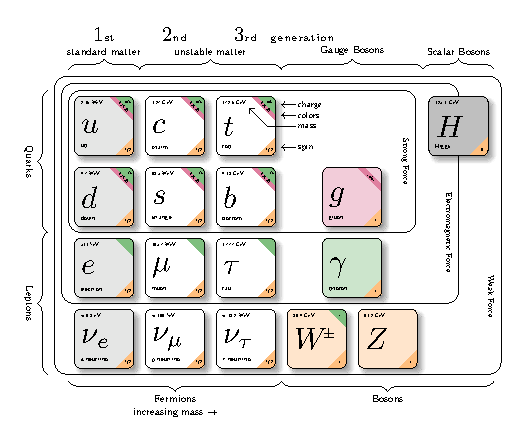
\includegraphics[width=0.8\textwidth]{figures/standard_model_pdf.pdf}
    \caption{Visualisation of The Standard Model of Particle Physics taken from~\cite{texample_model_physics} and modified with values taken from~\cite{pdg2025}}\label{fig:standard_model}
\end{figure}
\\